\chapter{Phân tích và thiết kế hệ thống}

\section{Phân tích yêu cầu}
    \subsection{Yêu cầu người dùng}
    	\begin{itemize}
				\item Đối với người dùng
					\begin{itemize}
				        \item Đăng kí, đăng nhập đổi mât khẩu cho người dùng.
				        \item Chỉnh sửa thông tin cá nhân: Người dùng có thể dễ dàng thay đổi thông tin cá nhân của mình.
				        \item Tạo đơn hàng: Lúc tạo đơn hàng người dùng có thể tự đến gửi hàng trực tiếp tại kho hoặc người dùng chọn option có tài xế đên lấy, phí vận chuyển có thể là người gửi thanh toán hoặc người nhận thanh toán.
				        \item Hủy đơn hàng: Trong khoảng thời gian đơn hàng được xác nhận bởi tài xế thì đơn hàng có thể bị hủy. Chú ý rằng sau khi đơn hàng đã được xác nhận thì người dùng không thể hủy, nếu bắt buộc phải hủy thì người dùng vẫn phải chịu chi phí vận chuyển.
				        \item Xem danh sách các đơn hàng: Người dùng có thể dễ dàng xem thông tin đơn hàng. Danh sách đơn hàng có thể được lọc theo trạng thái, theo mã đơn hàng hoặc theo từng khoảng thời gian khác nhau nhanh chóng.
				        \item Xem nợ công và thanh toán: Người dùng có thể xem các đơn hàng đã hoàn tất và tiến hành thanh toán trung gian qua Ví điện tử hoăc thẻ ngân hàng.
				        \item Nhận thông báo: Sau khi đơn hàng được xác nhận bởi tài xế, thì ngươi dùng sẽ liên tục nhận được thông báo mỗi khi chuyển trạng thái của đơn hàng. Điều này giúp cho người dùng có thể theo dõi đơn hàng chặt chẽ và dễ dàng dự báo thời gian nhận hàng của mình.
				        \item Tìm kiếm đơn hàng: Đối với người nhận không phải là user của hệ thống thì vẫn có thể dễ dàng xem thông tin các đơn hàng thông qua số điện thoại của mình hoặc theo dõi yêu cầu thông qua mã yêu cầu.
				        \item Yêu cầu hỗ trợ: Khi có các vấn đề thắc mắc thì người dùng có thể gửi yêu cầu để quản lý trực tiếp phản hồi. Danh sách các yêu cầu có thể được lọc theo mã yêu cầu, ngày, tháng, năm.
				        
				    \end{itemize}
				
			         
				\item Đối với tài xế
	                \begin{itemize}
	                    \item Đăng nhập đổi mât khẩu cho tài xế.
	                    \item Chỉnh sửa thông tin cá nhân: Tài xế có thể dễ dàng thay đổi thông tin cá nhân của mình.
	                    \item Nhận đơn hàng: Sau khi đơn hàng được tạo ra thì tài xế có thể nhận đơn và tiến hành vận chuyển hàng hóa.
	                    \item Xem danh sách kiện hàng cần lấy: Hệ thống sẽ tự động gán đơn đối với tài xế liên tỉnh và tài xế đi giao cho nên tài xế cần theo dõi danh sách đơn hàng cần lấy để lấy đúng kiện hàng mà mình vận chuyển.
	                    \item Xem danh sách kiện hàng cần giao: Tài xế có thể xem thông tin chi tiết về các đơn hàng mà mình cần giao.
	                    \item Xác nhận đơn hàng với người dùng: Trong quá trình giao nhận hàng giữa tài xế và người dùng (người nhận, người gửi) thì tài xế đều phải xác nhận đơn hàng để 
	                    \item Báo cáo vấn đề: Trong quá trình vận chuyển có thể xảy ra các vấn đề ngoài ý muốn như: làm thất lạc hàng, gặp sự cố ngoài ý muốn không thể đảm bảo thời gian giao hàng,... thì tài xế có thể báo cáo lên để quản lý có thể giải quyết.
	                    \item Nhận thông báo: Mỗi khi đơn hàng được gán cho tài xế thì sẽ có mail thông báo cho tài xế. Việc nay giúp tài xế nắm thông tin đơn hàng, đảm bảo việc giao nhận diễn ra kịp thời.
	                \end{itemize}
	                
	                
				\item Đối với thủ kho
			    	\begin{itemize}
			    	    \item Đăng nhập đổi mât khẩu cho thủ kho.
			    	    \item Chinh sửa thông tin thủ kho.
	                    \item Nhập kho: Sau khi đơn hàng vận chuyển đến kho thì thủ kho có trách nhiệm xác nhận đơn hàng đúng về số lượng và đảm bảo chất lượng nguyên vẹn. Sau khi xác nhận thì tiến hành nhập kho để lưu trữ và phân phối tiếp tục cho tài xế.
	                    \item Xuất kho: Sau khi đơn hàng đã phân phối cho tài xế thì thủ kho có trách nhiệm kiểm tra hàng một lần nữa và bàn giao cho tài xế. 
	                    \item Xuất hóa đơn: Trong quá trình nhập kho và xuất kho thì thủ kho có thể xuất hóa đơn để xác nhận đã nhập hàng hoặc bàn giao hàng hóa cho tài xế.
	                    \item Xem danh sách đơn hàng: Thủ kho có thể xem danh sách đơn hàng đang ở trong kho mà mình quản lý. Danh sách đơn hàng được lọc theo mã hoặc có thể theo ngày, tháng, năm.
	                    \item Xem lịch sử nhập xuất: Thủ kho có thể xem lịch sử nhập xuất đơn hàng vào/ra kho.
	                \end{itemize}
	                
	                
				\item Đối với quản lý
				    \begin{itemize}
	                    \item Đăng nhập đổi mât khẩu cho quản lý.
	                    \item Tạo tài khoản cho tài xế: Quản lý có thể tạo tài khoản và phân kho cho tài xế khi tài xế mới nhận việc.
	                    \item Xem biểu đồ thống kê: Quản lý có thể xem biểu đồ thống kê về tình hình hoạt động của các kho, tình hình vận chuyển hàng hóa.
	                    \item Xử lý sự cố: Khi nhận được sự cố từ tài xế thì quản lý có thể xử lý sự cố và cập nhật trạng thái đơn hàng cho người dùng.
	                    \item Xử lý yêu cầu từ người dùng: Khi người dùng yêu cầu thì quản lý có thể phản hồi thắc mắc hoặc các phản ánh tử người dùng.
	                \end{itemize}
		\end{itemize}
    
    \subsection{Yêu cầu hệ thống}
    Hệ thống vận chuyển hàng hóa liên tỉnh cần đáp ứng một số yêu cầu về hệ thống như sau:
        \begin{itemize}
            \item Thời gian xử lý mỗi request từ người dùng không quá 1s.
            \item Hệ thống gửi thông báo cho người dùng hoặc tài xế  không quá 5s.
            \item Hệ thống có thể chịu tải 100req/s.
            \item Thời gian tải hóa đơn nhập hàng/xuất hàng không quá 2s.
            \item Hệ thống cần mã hóa thông tin giao tiếp giữa client và server.
            \item Hệ thống phải được thiết kế để khi có nhu cầu mở rộng, thêm tính năng mới phải dễ dàng.
            \item Hệ thống cần xuất thống kê về số lượng đơn hàng được vận chuyển thành công, thất bại, doanh thu vào ngày cuối cùng trong tháng.
        \end{itemize}
    
    \newpage

\section{Thiết kế hệ thống}

\subsection{Kiến trúc hệ thống}
	
		\begin{figure}[H]
			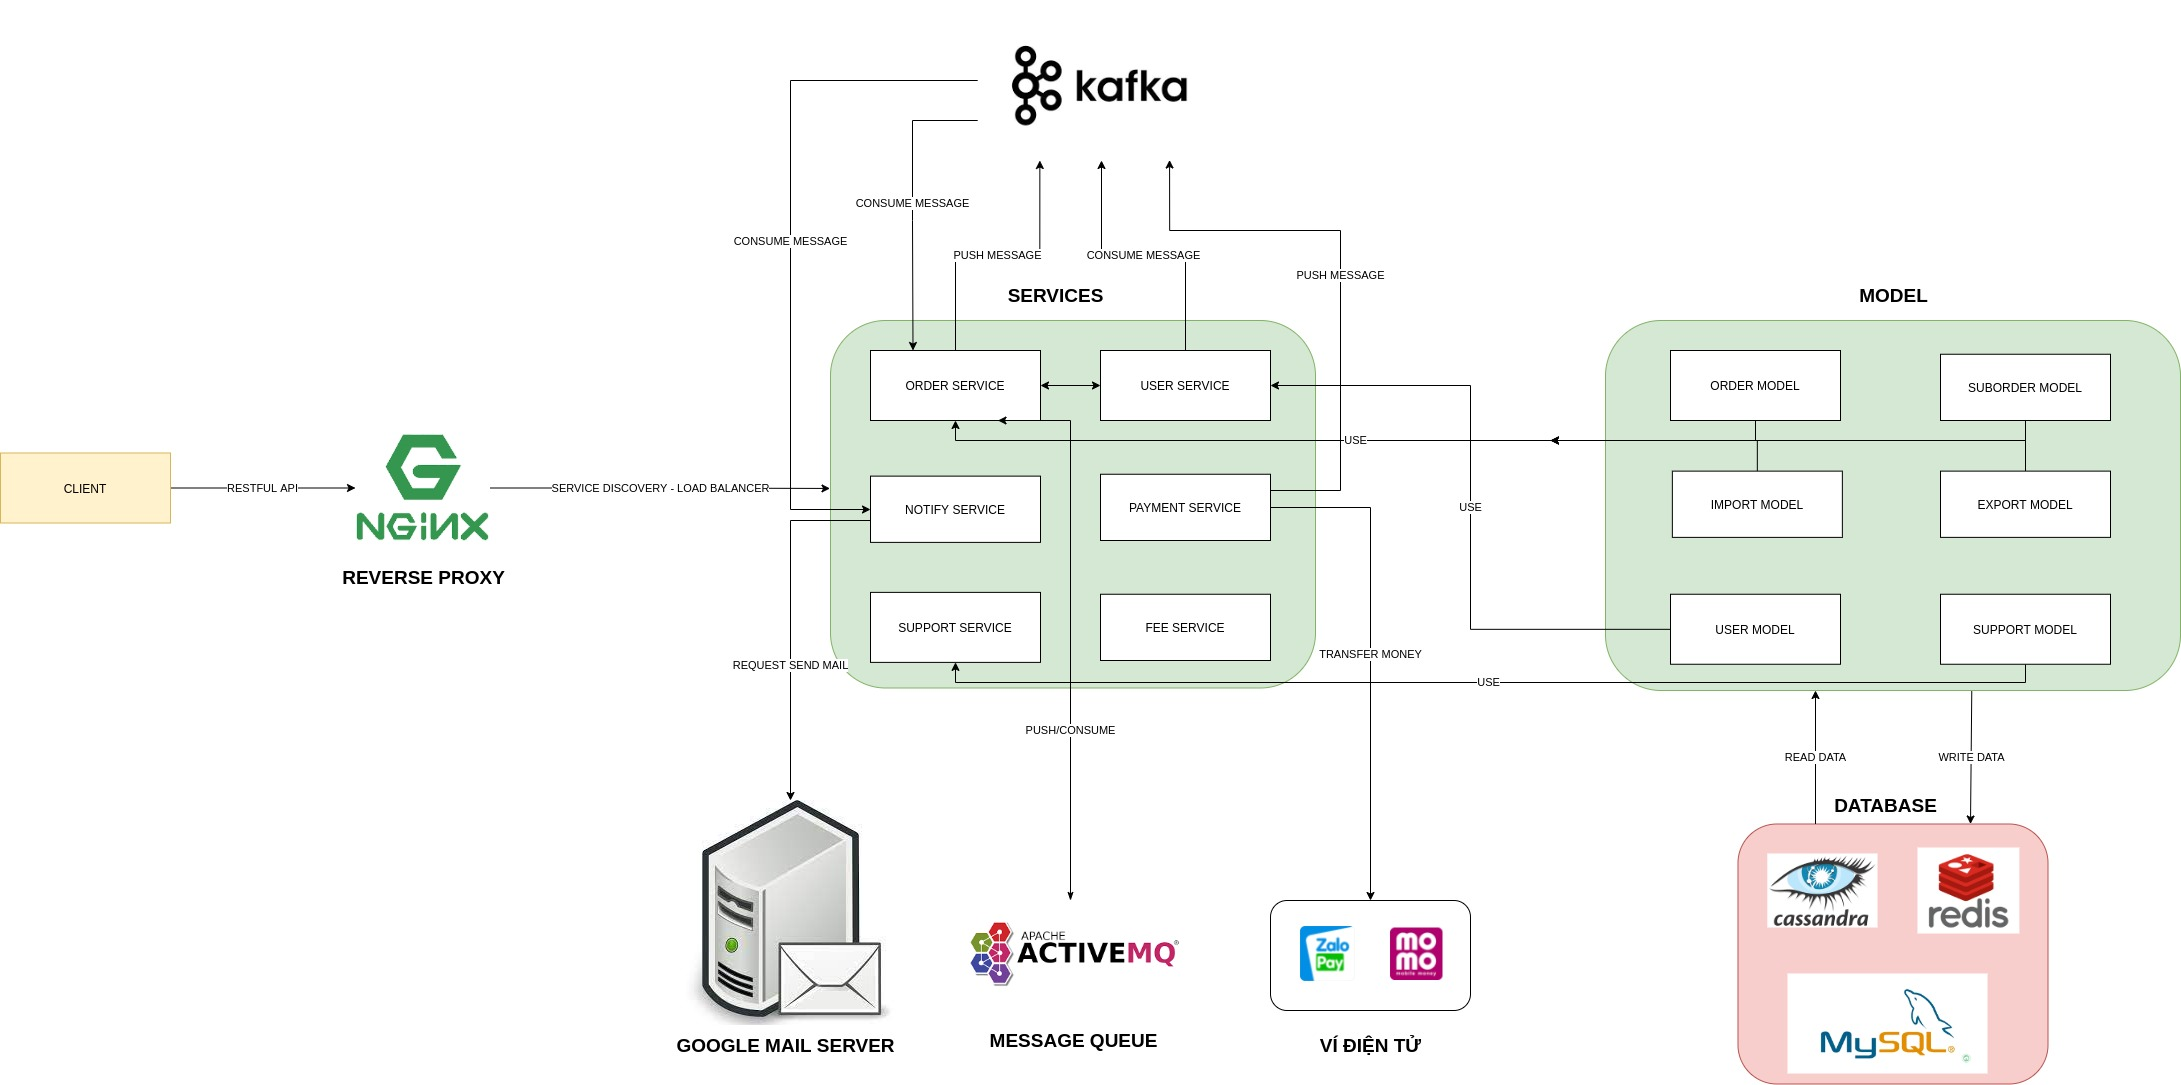
\includegraphics[width=1\textwidth]{Images/SystemArchitecture.jpg}
			\centering
			\linebreak
			\caption{Kiến trúc hệ thống}
		\end{figure}
	

		
		\begin{itemize}
			\item \textbf{User Service}
			\begin{itemize}
				\item Service chịu trách nhiệm quản lý user trong hệ thống. Ở đây sẽ lưu trữ Database của user
				\item Mỗi khi user login vào hệ thống thì sẽ vào Service này để authen: Ban đầu user được yêu cầu sẽ nhập username và password, Sau khi authen là đúng user đó thì hệ thống sẽ sinh ra JWT (Json Web Token) để gửi trả về cho user. Sau này cứ mỗi request lên hệ thống thì user sẽ gửi kèm theo JWT để hệ thống có thể authen và author.
				\item User có thể get thông tin để có thể xem và chỉnh sửa
			\end{itemize}
			\item \textbf{Order Service}
			\begin{itemize}
				\item Service chịu trách nhiệm tạo, xử lý, lưu trữ các thông tin về đơn hàng cho User.
				\item Ngoài ra service còn chịu trách nhiệm phân phối các đơn hàng đến tài xế
				\item Đây là service chịu tải khá lớn trong hệ thống vì nhóm sử dụng kết hợp các giải pháp sau nhằm tăng hiệu suất cho service: 
					\begin{itemize}
						\item Sử dụng Message Queue để hiện thực cơ chế bất đồng bộ cho các tác vụ: Tạo đơn hàng, ghi dữ liệu vào Database.
						\item Sử dụng Kafka để gửi message cho service khác
						\item Trong quá trinh xử lý thì dữ liệu của đơn hàng được lưu trên Cache. Đến khi nào có \textbf{trạng thái cuối} thì đơn hàng mới được lưu vào Database. Bởi vì đơn hàng đươc lấy và thay đổi trạng thái rất nhiều lần trong quá trình xử lý, nếu ghi vào Database (thực hiện nhiều I/O operations) sau mỗi lần xử lý như vậy thì sẽ làm giảm performance rất nhiều. Việc xử lý dữ liệu trên Cache cũng có thể gặp rủi ro như Cache Server sập thì dữ liệu có thể mất hết, nhưng rất may Redis có hỗ trợ cơ chế Persistence (định kỳ sao lưu dữ liệu) nên rủi ro này có thể chấp nhận được.
					\end{itemize}
				\item Mỗi khi đơn hàng thay đổi trạng thái hoăc tài xế đươc phân phối đơn thì service sẽ produce message vào \textbf{Kafka Broker} để \textbf{Notify Service} consume và tiếp tục xử lý
			\end{itemize}
			\item \textbf{Notify Service}
			\begin{itemize}
				\item Service chịu trách nhiệm quản lý các thông báo cho hệ thống.
				\item Service sẽ consume message tử \textbf{Order Service} và gửi yêu cầu về mail cho \textbf{Google Mail Server}.
				\item Hệ thống sẽ gửi thông báo mỗi khi: 
					\begin{itemize}
						\item Gửi thông báo cho khách hàng mỗi khi trạng thái đơn hàng thay đổi. 
						\item Gửi thông báo cho tài xế mỗi khi được phân phối đơn.
						\item Gửi mã xác thực OTP
					\end{itemize}
			\end{itemize}
			\item \textbf{Fee Service}
			\begin{itemize}
				\item Service chịu trách nhiệm hiện thực giải thuât, công thức để tính toán các khoản phí phát sinh cho khách hàng.
				\item Database lưu thông tin về phí của mỗi đơn hàng để các user có thể đối soát.
			\end{itemize}
			\item \textbf{Payment Service}
			\begin{itemize}
				\item Service này sẽ liên kết với 1 bên thứ 3 như: ngân hàng, ví điện từ, .... để thực hiện chức năng thanh toán cho các user.
			\end{itemize}
			\item \textbf{Reverse Proxy}
			\begin{itemize}
				\item Hệ thống sử dụng NGINX như là một \textbf{Reverse Proxy} nhằm thực hiện một số chức năng như: 
				\begin{itemize}
					\item \textbf{Bảo mât}: Kiểm soát các yêu cầu của Client gửi tới, nếu hợp lệ sẽ luân chuyển đến các service bên trong để xử lý. Che giấu địa chỉ IP của các service bên trong nhằm giúp các service trách khỏi các cuôc tấn công mạng. Ngoài ra còn có thể dễ dàng thiết lập SSL nhằm mã hóa dữ liệu trong quá trình giao tiếp giữa Client và các service bên trong.
					\item \textbf{Cân bằng tải}: Mỗi service có thể được deploy với nhiều instance để có thể chịu tải cao hơn. Reverse proxy sẽ thực hiện một số giải thuật như: Round Robin, Least Connection, ... để đẩy các request vào cho các service xử lý.
				\end{itemize}
			\end{itemize}
			
				\item \textbf{Database}
				\begin{itemize}
					\item \textbf{MySQL}: Hệ thống sử dụng MySql để lưu các thông tin ít được truy xuất như log, cấu hình service,...
					\item \textbf{Cassandra}: Với khả năng đọc/ghi có tốc độ nhanh cùng với đó là khả năng chịu lỗi cao hệ thống sử dụng Cassandra để lưu các thông tin về Order, Hóa đơn nhập/xuất kho,...
					\item \textbf{Redis}: Với Redis thì dữ liệu được lưu trữ trong memory vì thế giúp cho service truy xuất thông tin rất nhanh chóng. Hệ thống sẽ lưu các thông tin thường xuyên được truy xuất bởi user như thông tin về yêu cầu, đơn hàng,... Ngoài ra còn tận dụng cấu trúc dữ liệu đa dạng trong Redis để giải quyết một số bài toán phức tạp. 
				\end{itemize}
		
		\end{itemize}

\newpage
\subsection{Thiết kế và đặc tả Use Case}

\begin{figure}[H]
	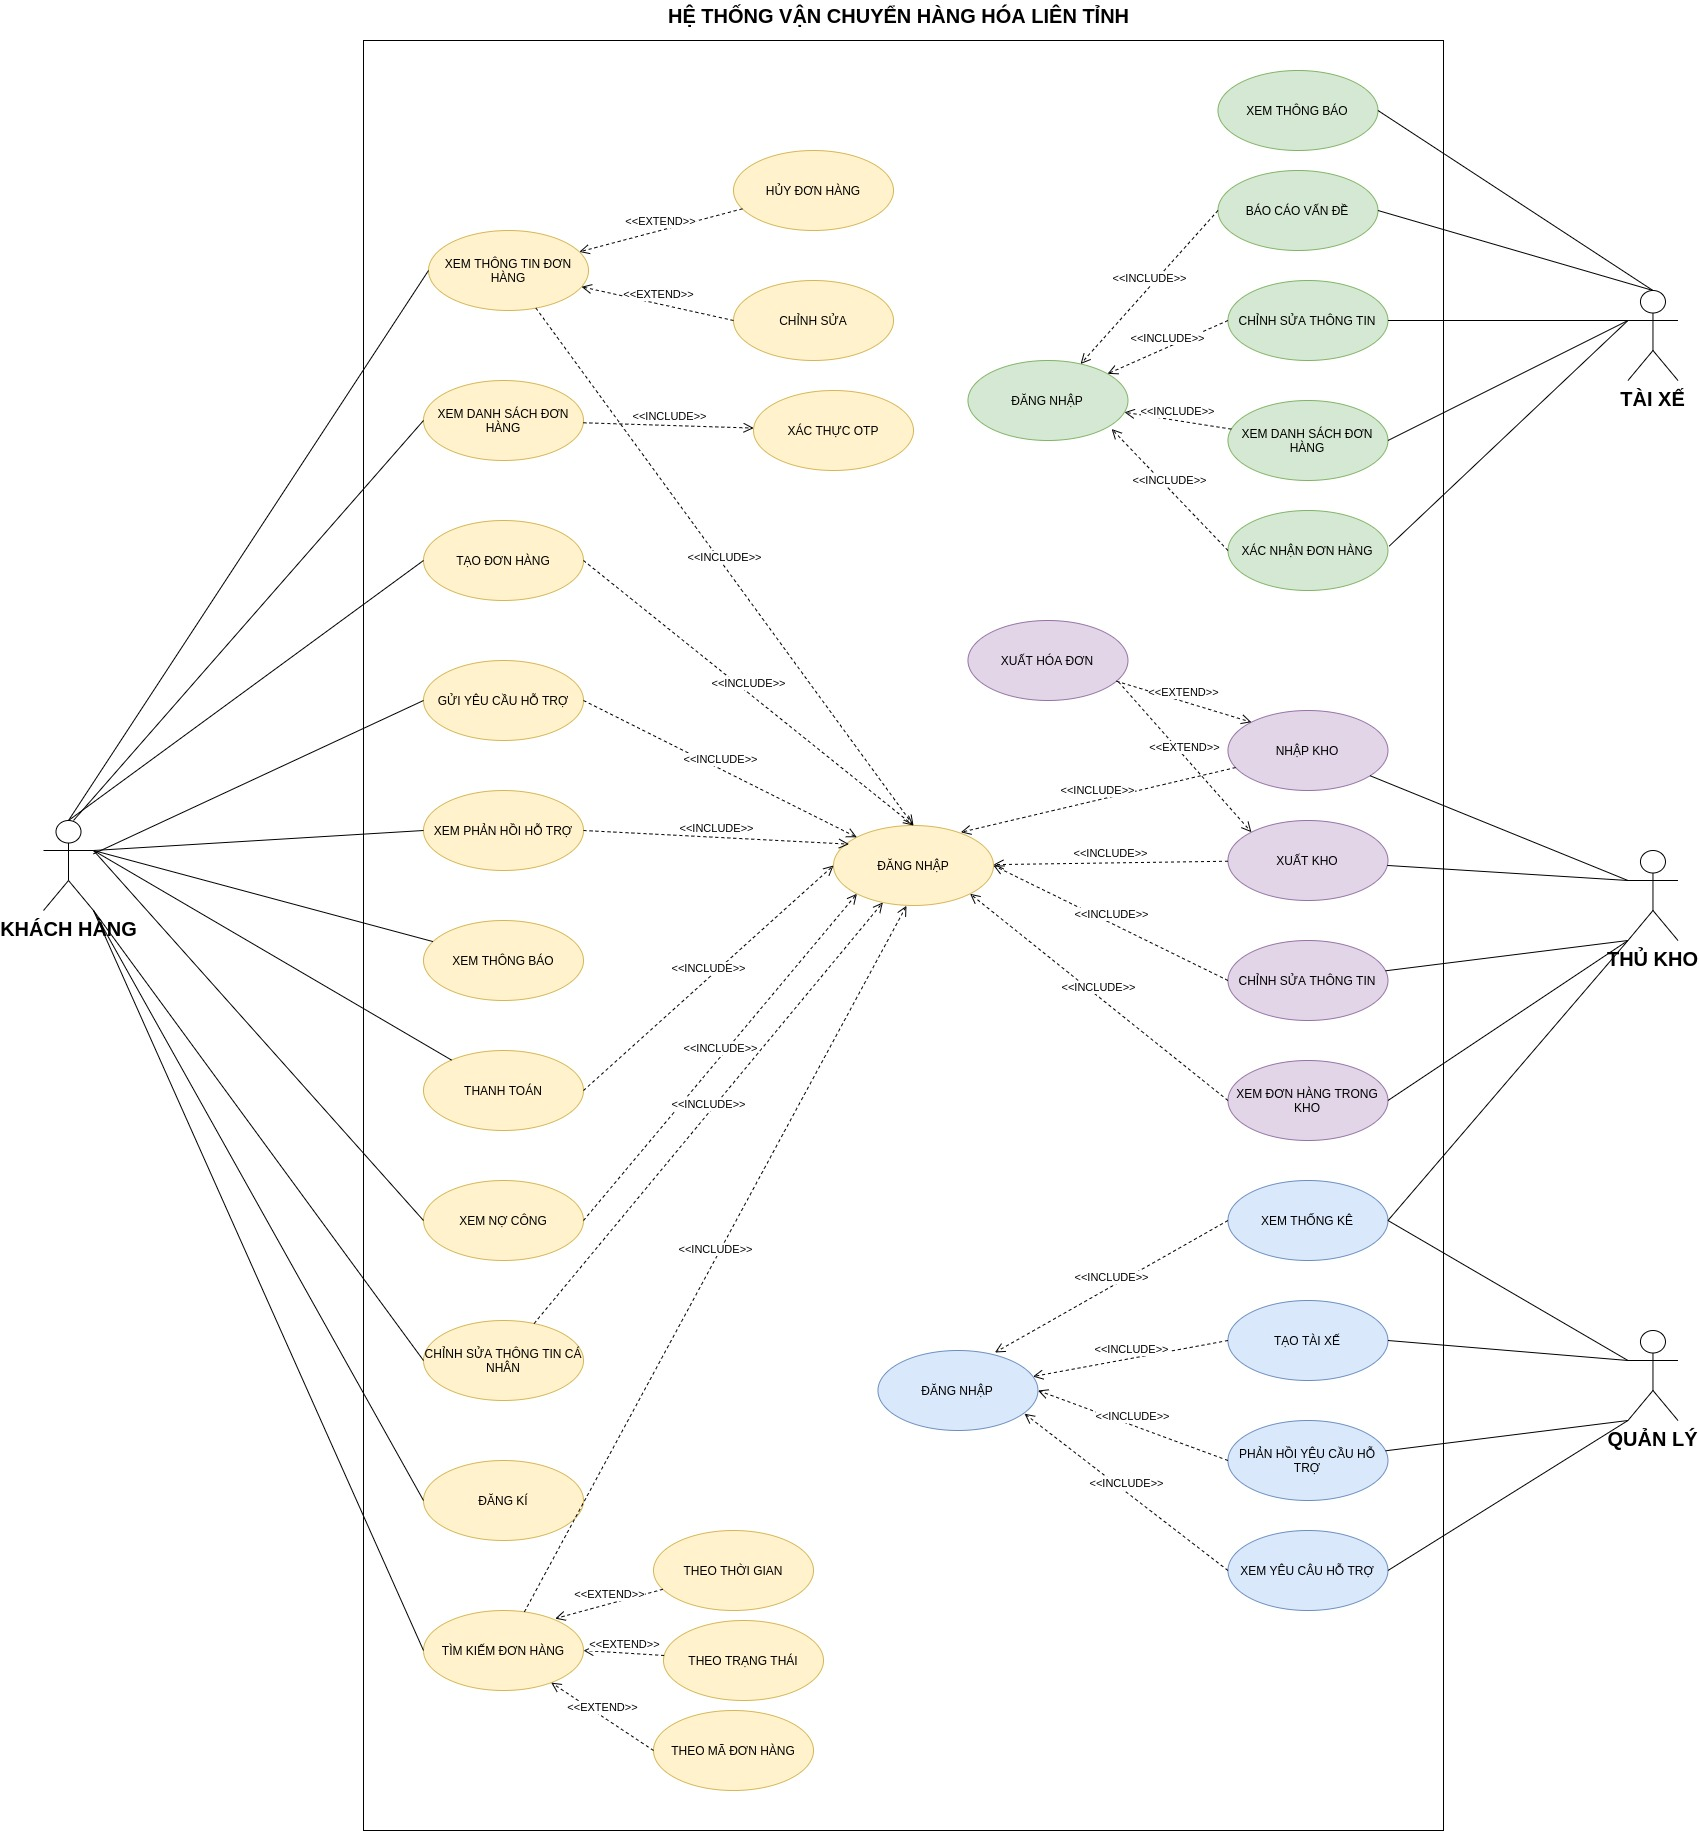
\includegraphics[width=1\textwidth]{/UseCase.jpg}
	\centering
	\linebreak
	\caption{Sơ đồ Use case}
\end{figure}

	\newpage
	
	\begin{itemize}
		\item \textbf{Use case cho Khách Hàng}
		\begin{itemize}
			\item \textbf{Tạo đơn hàng:} Người gửi cần điền những thông tin sau: 
			\begin{itemize}
				\item Bên gửi: Hệ thống sẽ tự động nhập thông tin khi người gửi đăng nhập bao gồm:
				\begin{itemize}
					\item Tên người gửi
					\item Số điện thoại
					\item Địa chỉ, chia làm 4 phần gồm Số địa chỉ + tên đường, Phường - Xã, Quận - Huyện, Thành phố - Tỉnh. 
				\end{itemize}
				\item Bên nhận:
				\begin{itemize}
					\item Tên người nhận
					\item Số điện thoại
					\item Địa chỉ, tương tự như bên gửi. Khi người gửi nhập địa chỉ hệ thống sẽ tự động lấy chính xác địa chỉ thông qua Google Map API.
				\end{itemize}
				\item Thông tin về món hàng muốn gửi:
				\begin{itemize}
					\item Loại hàng hóa
					\item Khối lượng (Để tính phí vận chuyển). Nhân viên đến lấy hàng sẽ tiến hành xác nhận bằng cách đo lại và sẽ yêu cầu khách hàng cập nhật lại khối lượng nếu như khối lượng đã nhập trước đó là không chính xác.
					\item Giá trị hàng hóa (VND): Giá trị ước tính của hàng hóa để đền bù khi gặp sự cố.
					
				\end{itemize}
				\item Lựa chọn tính phí cho bên gửi hoặc bên nhận 
				\item Lựa chọn gửi hàng/nhận hàng tại kho sẽ không tính phí nội tỉnh (phí liên tỉnh luôn có). Ngược lại sẽ tính phí nội tỉnh (gửi và nhận giống nhau). 
				\item Hệ thống sẽ tự tính cước vận chuyển dựa trên khoảng cách bên gửi/nhận và khối lượng món hàng.
				\item Các thông tin ghi chú khác (Người gửi tự điền vào ô textbox).
			\end{itemize} 
				
			
			
				\begin{table}[H]
					\centering\begin{tabular}{|c|m{25em}|}
						\hline 
						Use case name & Tạo đơn hàng\\ 
						\hline 
						Actors & Khách hàng \\ 
						\hline
						Description & Người dùng có thể tạo đơn hàng của mình \\
						\hline 
						Preconditions & Người dùng đã đăng nhập vào hệ thống \\
						\hline
						Postconditions & Đơn hàng được tạo ra, các thông tin về đơn hàng được lưu trữ, đơn hàng sẽ được gán cho tài xế đến lấy (nếu người dùng không đến kho gửi hàng) \\
						\hline
						Nomar Flow & \begin{enumerate}
											\item Ở trang chủ khách hàng chọn Tab "Quản lý đơn hàng".
											\item Chọn "Lên đơn hàng" ở góc trên bên trái màn hình.
											\item Nhập đầy đủ các thông tin yêu cầu.
											\item Nhấn "Tạo đơn".
									\end{enumerate}
							\\
						\hline
					\end{tabular}
					\caption{Tạo đơn hàng}
				\end{table}
			
			\item \textbf{Xem đơn hàng được nhận}: Người nhận có thể nhập số điện thoại để xem các đơn hàng được nhận, các đơn hàng sẽ được chia theo trạng thái đã định nghĩa ở trên và người gửi có thể xem list các đơn hàng lọc theo trạng thái đó. 
			
			
			\begin{table}[H]
				\centering\begin{tabular}{|c|m{25em}|}
					\hline 
					Use case name & Xem đơn hàng được nhận\\ 
					\hline 
					Actors & Người nhận \\ 
					\hline
					Description & Nguời nhận có thể xem đơn hàng được nhận thông qua số điện thoại mà không cần đăng nhập \\
					\hline 
					Preconditions & Thông tin đơn hàng phải có số điện thoại và email của người nhận \\
					\hline
					Postconditions & Danh sách đơn hàng được hiển thị cho người nhận \\
					\hline
					Nomar Flow & \begin{enumerate}
						\item Ở trang landing page người nhận chọn "Xem danh sách đơn hàng".
						\item Nhập số điện thoại.
						\item Nhập mã OTP nhận được thông qua Email.
					\end{enumerate}
					\\
					\hline
				\end{tabular}
				\caption{Xem đơn hàng được nhận}
			\end{table}
		
		
		\item \textbf{Xem thông tin đơn hàng:} Khách hàng có thể xem thông tin đơn hàng theo các trạng thái khác nhau, theo mã đơn hàng hoặc theo khoảng thời gian nào đó.
			
			\begin{table}[H]
				\centering\begin{tabular}{|c|m{25em}|}
					\hline 
					Use case name & Xem thông tin đơn hàng\\ 
					\hline 
					Actors & Khách hàng \\ 
					\hline
					Description & Khách hàng xem thông tin đơn hàng sau khi đã đăng nhập vào hệ thống \\
					\hline 
					Preconditions & Khách hàng đã đăng nhập vào hệ thống \\
					\hline
					Postconditions & Danh sách đơn hàng được hiển thị. Khách hàng có thể lọc đơn hàng theo mã đơn hàng, trạng thái, ngày tháng. \\
					\hline
					Nomar Flow & \begin{enumerate}
						\item Ở trang chủ nhấn "Quản lí đơn hàng". Mặc định sẽ hiển thị tất cả đơn hàng của khách hàng đó.
						\item Khách hàng có thể lọc theo các tiêu chí khác nhau nếu cần
					\end{enumerate}
					\\
					\hline
				\end{tabular}
				\caption{Xem thông tin đơn hàng}
			\end{table}
			
			\item \textbf{Hủy đơn hàng:} Nếu vẫn đang trong quá trình bàn giao và xác nhận(trong trạng thái \textbf{Chờ bàn giao}), thì người gửi có thể hủy đơn hàng nếu muốn.
			
			
			\begin{table}[H]
				\centering\begin{tabular}{|c|m{25em}|}
					\hline 
					Use case name & Hủy đơn hàng\\ 
					\hline 
					Actors & Người gửi \\ 
					\hline
					Description & Người gửi có thể hủy nếu đơn hàng chưa đươc bàn giao cho tài xế. \\
					\hline 
					Preconditions & Người gửi đã đăng nhập vào hệ thống \\
					\hline
					Postconditions & Đơn hàng bị hủy \\
					\hline
					Nomar Flow & \begin{enumerate}
						\item Ở trang chủ nhấn "Quản lí đơn hàng". Mặc định sẽ hiển thị tất cả yêu cầu của khách hàng đó.
						\item Tại đơn hàng khách hàng nhấn vào "Hủy đơn hàng".
						\item Nhấn "Xác nhận".
					\end{enumerate}
					\\
					\hline
				\end{tabular}
				\caption{Hủy đơn hàng}
			\end{table}
			
			\item \textbf{Gửi yêu cầu hỗ trợ:} Trong quá trinh vận chuyển nếu có thắc mắc nào thì khách hàng có thể gửi yêu cầu để quản lý hỗ trợ.
			
			\begin{table}[H]
				\centering\begin{tabular}{|c|m{25em}|}
					\hline 
					Use case name & Gửi yêu cầu hỗ trợ\\ 
					\hline 
					Actors & Khách hàng \\ 
					\hline
					Description & Khách hàng gửi yêu cầu và quản lý sẽ trực tiếp phản hồi yêu cầu đó. \\
					\hline 
					Preconditions & Khách hàng đã đăng nhập vào hệ thống \\
					\hline
					Postconditions & Yêu cầu được submit và chờ quản lý phản hồi \\
					\hline
					Nomar Flow & \begin{enumerate}
						\item Ở trang chủ nhấn "Yêu cầu hỗ trợ".
						\item Nhấn "Lên yêu cầu".
						\item Nhập các thông tin cần thiết như: Mã đơn hàng, trình bày nội dung cần hỗ trợ.
						\item Nhấn "Xác nhận".
					\end{enumerate}
					\\
					\hline
				\end{tabular}
				\caption{Gửi yêu cầu hỗ trợ}
			\end{table}
		
			\item \textbf{Xem phản hồi hỗ trợ}: Sau khi yêu cầu hỗ trợ được phản hồi bởi quản lý thì khách hàng có thể xem thông tin phản hồi đó.
			
			\begin{table}[H]
				\centering\begin{tabular}{|c|m{25em}|}
					\hline 
					Use case name & Xem phản hồi hỗ trợ\\ 
					\hline 
					Actors & Khách hàng \\ 
					\hline
					Description & Khách hàng xem yêu cầu hỗ trợ được phản hồi bởi quản lý \\
					\hline 
					Preconditions & Khách hàng đã đăng nhập vào hệ thống \\
					\hline
					Postconditions & Hiển thị danh sách yêu cầu phản hồi \\
					\hline
					Nomar Flow & \begin{enumerate}
						\item Ở trang chủ nhấn "Yêu cầu hỗ trợ". Mặc định sẽ hiển thị ra thông tin các yêu cầu và phản hồi của quản lý (nếu yêu cầu đã đươc xử lý)
						\item Khách hàng có thẻ lọc yêu cầu theo: Mã yêu cầu, ngày tháng.
				
					\end{enumerate}
					\\
					\hline
				\end{tabular}
				\caption{Xem phản hồi hỗ trợ}
			\end{table}
			
			\item \textbf{Xem thông báo}: Mỗi khi trạng thái đơn hàng thay đổi thì khách hàng đều nhận được email thông báo để khách hàng có thể nắm bắt đươc tình trạng của đơn hàng. Ngoài ra môt số chức năng cần phải nhập OTP để xác thực khách hàng thì cũng được gửi thông qua email.
			
			\begin{table}[H]
				\centering\begin{tabular}{|c|m{25em}|}
					\hline 
					Use case name & Xem thông báo\\ 
					\hline 
					Actors & Khách hàng \\ 
					\hline
					Description & Khách hàng xem thông báo của mình thông qua Email \\
					\hline 
					Preconditions & Khách hàng đã đăng nhập vào email của mình \\
					\hline
					Postconditions & Khách hàng xem đươc thông báo của mình từ BKShipment \\
					\hline
					Nomar Flow & \begin{enumerate}
						\item Người dùng đăng nhập Email của mình
						\item Mở hộp thư đến
						
					\end{enumerate}
					\\
					\hline
				\end{tabular}
				\caption{Xem thông báo}
			\end{table}
		
			\item \textbf{Xem nợ công}: Sau khi đơn hàng được xác nhận là hoàn thành thì sẽ có thống kê về nợ công để khách hàng dễ dàng quan sát và thanh toán.
			
			\begin{table}[H]
				\centering\begin{tabular}{|c|m{25em}|}
					\hline 
					Use case name & Xem nợ công\\ 
					\hline 
					Actors & Khách hàng \\ 
					\hline
					Description & Khách hàng có thể xem nợ công của mình \\
					\hline 
					Preconditions & Khách hàng đã đăng nhập vào hệ thống \\
					\hline
					Postconditions & Hiển thị danh sách nợ công với tương ứng với các đơn hàng của người dùng \\
					\hline
					Nomar Flow & \begin{enumerate}
						\item Ở trang chủ nhấn "Thanh toán". Mặc định sẽ hiển thị ra thông tin các đơn hàng đã hoàn thành và số tiền phải thanh toán.
					
						
					\end{enumerate}
					\\
					\hline
				\end{tabular}
				\caption{Xem nợ công}
			\end{table}
		
			\item \textbf{Thanh toán}: Sau khi xem xét nợ công của các đơn hàng thì khách hàng có thể tiến hành thanh toán chi phí cho doanh nghiệp. Khách hàng có thể thanh toán từng đơn hàng hoặc chọn nhiều đơn hàng cùng một lúc.
			
			\begin{table}[H]
				\centering\begin{tabular}{|c|m{25em}|}
					\hline 
					Use case name & Thanh toán\\ 
					\hline 
					Actors & Khách hàng \\ 
					\hline
					Description & Khách hàng thanh toán đơn hàng thông qua trung gian là Ví điện tử \\
					\hline 
					Preconditions & Khách hàng đã đăng nhập vào hệ thống \\
					\hline
					Postconditions & Đơn hàng đã được thanh toán. Tiền trong ví điện tử của khách hàng được trả cho doanh nghiệp. \\
					\hline
					Nomar Flow & \begin{enumerate}
						\item Ở trang chủ nhấn "Thanh toán". Mặc định sẽ hiển thị ra thông tin các đơn hàng đã hoàn thành và số tiền phải thanh toán.
						\item Khách hàng có thể lựa chọn từng đơn hàng hoặc nhiều đơn hàng.
						\item Chọn phương thức thanh toán.
						\item Nhấn "Xác nhận".
						
					\end{enumerate}
					\\
					\hline
				\end{tabular}
				\caption{Thanh toán}
			\end{table}
		
			\item \textbf{Chỉnh sửa thông tin cá nhân}: Khách hàng có thể thay đổi một số thông tin cá nhân khi cần thiết.
			
				\begin{table}[H]
					\centering\begin{tabular}{|c|m{25em}|}
						\hline 
						Use case name & Chỉnh sửa thông tin cá nhân\\ 
						\hline 
						Actors & Khách hàng \\ 
						\hline
						Description & Khách hàng có thể thay đổi thông tin cá nhân của mình. \\
						\hline 
						Preconditions & Khách hàng đã đăng nhập vào hệ thống \\
						\hline
						Postconditions & Thông tin cá nhân của khách hàng được thay đổi. \\
						\hline
						Nomar Flow & \begin{enumerate}
							\item Ở trang chủ nhấn "Chỉnh sửa thông tin".
							\item Khách hàng có thể thay đổi một số thông tin như: Email, SĐT, tên tài khoản, địa chỉ, mật khẩu.
							\item Nhấn "Cập nhật".
							
						\end{enumerate}
						\\
						\hline
					\end{tabular}
					\caption{Chỉnh sửa thông tin cá nhân}
				\end{table}
			
		\end{itemize}
	
	
	\item \textbf{Use case cho Tài xế}
	
	\begin{itemize}
		\item \textbf{Xem thông báo}: Tương tự như Khách hàng thì khi mỗi đơn hàng được gán cho Tài xế thì sẽ có mail thông báo giúp cho tài xế tiếp nhận thông tin kịp thời.
		
		\item \textbf{Báo cáo vấn đề}: Trong quá trình vận chuyển có thể xảy ra các trường hợp ngoài ý muốn như mất hàng, chậm trễ việc chuyển hàng thì Tài xế có thể báo cáo vấn đề lên để Quản lý có thể giải quyết kịp thời.
		
		\begin{table}[H]
			\centering\begin{tabular}{|c|m{25em}|}
				\hline 
				Use case name & Báo cáo vấn đề\\ 
				\hline 
				Actors & Tài xế \\ 
				\hline
				Description & Tài xế báo cáo vấn đề lên Quản lý để xử lý \\
				\hline 
				Preconditions & Tài xế đã đăng nhập vào hệ thống \\
				\hline
				Postconditions & Nội dung vấn đề được gửi lên để chờ Quản lý xử lý. \\
				\hline
				Nomar Flow & \begin{enumerate}
					\item Ở trang chủ nhấn "Báo cáo vấn đề".
					\item Nhấn "Tạo yêu cầu".
					\item Nhập các thông tin cần thiết
					\item Nhấn "Gửi yêu cầu".
					
				\end{enumerate}
				\\
				\hline
			\end{tabular}
			\caption{Báo cáo vấn đề}
		\end{table}
	
		\item \textbf{Chỉnh sửa thông tin}: Tài xế có thể chính sửa một số thông tin khi có thay đổi.
		
		\item \textbf{Xem danh sách đơn hàng}: Tài xế có thể xem danh sách đơn hàng cần lấy, danh sách đơn hàng đã giao, đã hoàn thành, đã hủy,...
		
		\begin{table}[H]
			\centering\begin{tabular}{|c|m{25em}|}
				\hline 
				Use case name & Xem danh sách đơn hàng\\ 
				\hline 
				Actors & Tài xế \\ 
				\hline
				Description & Tài xế xem các thông tin về đơn hàng \\
				\hline 
				Preconditions & Tài xế đã đăng nhập vào hệ thống \\
				\hline
				Postconditions & Đơn hàng được hiển thị. Tài xế có thể lọc theo mã đơn hàng, ngày tháng, trạng thái. \\
				\hline
				Nomar Flow & \begin{enumerate}
					\item Ở trang chủ nhấn "Quản lý đơn hàng".
					\item Chọn tab "Đơn hàng cân lấy", "Đơn hàng đang giao", "Đơn hàng đã giao" để xem thông tin về đơn hàng cần biết.	
				\end{enumerate}
				\\
				\hline
			\end{tabular}
			\caption{Xem danh sách đơn hàng}
		\end{table}
	
		\item \textbf{Xác nhận đơn hàng}: Mỗi khi giao nhận hàng thì tài xế có nhiệm vụ phải kiểm tra kĩ tình trạng và số lượng của kiện hàng. Sau đó cần phải xác nhận lại với hệ thống và phải chịu hoàn toàn trách nhiệm nếu đơn hàng có sai sót về tình trạng và số lượng.
		
		\begin{table}[H]
			\centering\begin{tabular}{|c|m{25em}|}
				\hline 
				Use case name & Xác nhận đơn hàng\\ 
				\hline 
				Actors & Tài xế \\ 
				\hline
				Description & Tài xế xác nhận đơn hàng \\
				\hline 
				Preconditions & Tài xế đã đăng nhập vào hệ thống \\
				\hline
				Postconditions & Đơn hàng được xác nhận với hệ thống. Hệ thống lưu trữ lại thông tin mới nhất về đơn hàng. \\
				\hline
				Nomar Flow & \begin{enumerate}
					\item Ở trang chủ nhấn "Quản lý đơn hàng".
					\item Chọn đơn hàng cần xác nhận.
					\item Chỉnh sửa các thông tin sai sót nếu có.
					\item Nhấn "Xác nhận".
				\end{enumerate}
				\\
				\hline
			\end{tabular}
			\caption{Xác nhận đơn hàng}
		\end{table}
		
	\end{itemize}


	\item \textbf{Use case cho Thủ kho}
	
	\begin{itemize}
		\item \textbf{Nhập kho}: Sau khi hàng được vận chuyển về kho thì thủ kho chịu trách nhiệm kiểm tra lại tình trạng và số lượng của đơn hàng. Nếu không có vấn đề gì xảy ra thì thủ kho nhập hàng vào kho để lưu trữ và chờ phân phối cho tài xế.
		
		\begin{table}[H]
			\centering\begin{tabular}{|c|m{25em}|}
				\hline 
				Use case name & Nhập kho\\ 
				\hline 
				Actors & Thủ kho \\ 
				\hline
				Description & Thủ kho tiến hành nhập hàng hóa vào kho \\
				\hline 
				Preconditions & Thủ kho đã đăng nhập vào hệ thống. \\
				\hline
				Postconditions & Hàng đươc nhập vào kho. Thông tin nhập kho được lưu trữ lại để đối soát về sau. \\
				\hline
				Nomar Flow & \begin{enumerate}
					\item Ở trang chủ nhấn "Nhập kho".
					\item Nhập mã tài xế
					\item Chọn từng đơn hàng hoăc nhiều đơn hàng.
					\item Nhấn "Nhập hàng".
					\item Thủ kho có thể nhấn "Xuất hóa đơn" và bàn giao hóa đơn cho Tài xế để dễ dàng đối soát về sau.
				\end{enumerate}
				\\
				\hline
			\end{tabular}
			\caption{Nhập kho}
		\end{table}
	
		\item \textbf{Xuất kho}: Sau khi đơn hàng đươc phân phối cho tài xế. Thì tài xế đến kho nhận hàng và tiếp tục vận chuyển. Khi xuất hàng thủ kho có trách nhiệm kiểm tra hàng hóa về số lượng và tình trạng một lần nữa trước khi bàn giao cho Tài xế.
		
		\begin{table}[H]
			\centering\begin{tabular}{|c|m{25em}|}
				\hline 
				Use case name & Xuất kho\\ 
				\hline 
				Actors & Thủ kho \\ 
				\hline
				Description & Thủ kho tiến hành xuất hàng hóa để tài xế tiếp tục vận chuyển \\
				\hline 
				Preconditions & Thủ kho đã đăng nhập vào hệ thống. \\
				\hline
				Postconditions & Hàng đươc xuất kho giao cho Tài xế đi giao. Thông tin xuất kho được lưu trữ lại để đối soát về sau. \\
				\hline
				Nomar Flow & \begin{enumerate}
					\item Ở trang chủ nhấn "Xuất kho".
					\item Nhập mã tài xế
					\item Chọn từng đơn hàng hoăc nhiều đơn hàng.
					\item Nhấn "Xuất hàng".
					\item Thủ kho có thể nhấn "Xuất hóa đơn" và bàn giao hóa đơn cho Tài xế để dễ dàng đối soát về sau.
				\end{enumerate}
				\\
				\hline
			\end{tabular}
			\caption{Xuất kho}
		\end{table}
	
		\item \textbf{Chỉnh sửa thông tin}: Thủ kho có thể chỉnh sửa một số thông tin khi cần thiết.
		
		\item \textbf{Xem đơn hàng đang có trong kho}: Thủ kho có thể xem thông tin về các đơn hàng có trong kho mà mình đang quản lý.
		
		\item \textbf{Xem lịch sử nhập xuất kho}: Thủ kho có thể xem lịch sử nhập/xuất kho. Các thông tin bao gồm mã yêu cầu / đơn hàng, thông tin tài xế, thông tin thủ khon và thông tin chi tiết của đơn hàng.
		
	\end{itemize}
		
		\item \textbf{Use case cho Quản lý}
		
		\begin{itemize}
			\item \textbf{Xem thống kê}: Quản lý có thể xem thông tin thống kê về tình hình kinh doanh của của doanh nghiệp như: dòng tiền, nhân sự, số lương đơn hàng thành công, thất bại,...
			
			\item \textbf{Tạo tài xế}: Mỗi khi tài xế mới nhận việc làm thì quản lý có trách nhiệm tạo tài xế và chỉ định kho hoạt động cho tài xế.
			
			\begin{table}[H]
				\centering\begin{tabular}{|c|m{25em}|}
					\hline 
					Use case name & Tạo tài xế\\ 
					\hline 
					Actors & Quản lý \\ 
					\hline
					Description & Quản lý tạo tài xế để tài xế hoàn thành quá trình nhận việc. \\
					\hline 
					Preconditions & Quản lý đã đăng nhập vào hệ thống. \\
					\hline
					Postconditions & Tài xế được tạo thành công. Thông tin tài khoản và mật khẩu có thể được bàn giao cho tài xế. \\
					\hline
					Nomar Flow & \begin{enumerate}
						\item Ở trang chủ nhấn "Tạo tài xế".
						\item Nhập các thông tin cần thiết như: Kho hoạt động, phương tiện, mã phương tiện, ...
						\item Nhấn "Xác nhận".
					\end{enumerate}
					\\
					\hline
				\end{tabular}
				\caption{Tạo tài xế}
			\end{table}
		
			\item \textbf{Phản hồi yêu cầu hỗ trợ}: Sau khi nhận được yêu cầu hỗ trợ từ khách hàng thì quản lý có trách nhiệm phản hồi, giải đáp các yêu cầu, thắc mắc của khách hàng.
			
			\begin{table}[H]
				\centering\begin{tabular}{|c|m{25em}|}
					\hline 
					Use case name & Phản hồi yêu cầu hỗ trợ\\ 
					\hline 
					Actors & Quản lý \\ 
					\hline
					Description & Quản lý có thể phản hồi yêu cầu hỗ trợ từ khách hàng. \\
					\hline 
					Preconditions & Quản lý đã đăng nhập vào hệ thống. \\
					\hline
					Postconditions & Yêu cầu được phản hồi và thông báo về khách hàng. \\
					\hline
					Nomar Flow & \begin{enumerate}
						\item Ở trang chủ nhấn "Danh sách yêu cầu".
						\item Chọn yêu cầu và nhập thông tin phản hồi.
						\item Nhấn "Xác nhận".
					\end{enumerate}
					\\
					\hline
				\end{tabular}
				\caption{Phản hồi yêu cầu hỗ trợ}
			\end{table}
		
			\item \textbf{Xử lý sự cố}: Sau khi nhận đươc thông tin có sự cố từ phía Tài xế thì Quản lý có trách nhiệm giải quyết các vấn đề. 
			
			\begin{table}[H]
				\centering\begin{tabular}{|c|m{25em}|}
					\hline 
					Use case name & Xử lý sự cố\\ 
					\hline 
					Actors & Quản lý \\ 
					\hline
					Description & Quản lý có thể xử lý sự cố bất ngờ từ tài xế. \\
					\hline 
					Preconditions & Quản lý đã đăng nhập vào hệ thống. \\
					\hline
					Postconditions & Sự cố đươc xử lý. Trạng thái đơn hàng đươc cập nhật. \\
					\hline
					Nomar Flow & \begin{enumerate}
						\item Ở trang chủ nhấn "Danh sách sự cố".
						\item Chọn sự cố, giải quyết và cập nhật trạng thái đơn hàng.
						\item Nhấn "Xác nhận".
					\end{enumerate}
					\\
					\hline
				\end{tabular}
				\caption{Xử lý sự cố}
			\end{table}
			
			
		\end{itemize}
	\end{itemize}
    
	
	\subsection{Thiết kế cơ sở dữ liệu}
	
		\begin{figure}[H]
			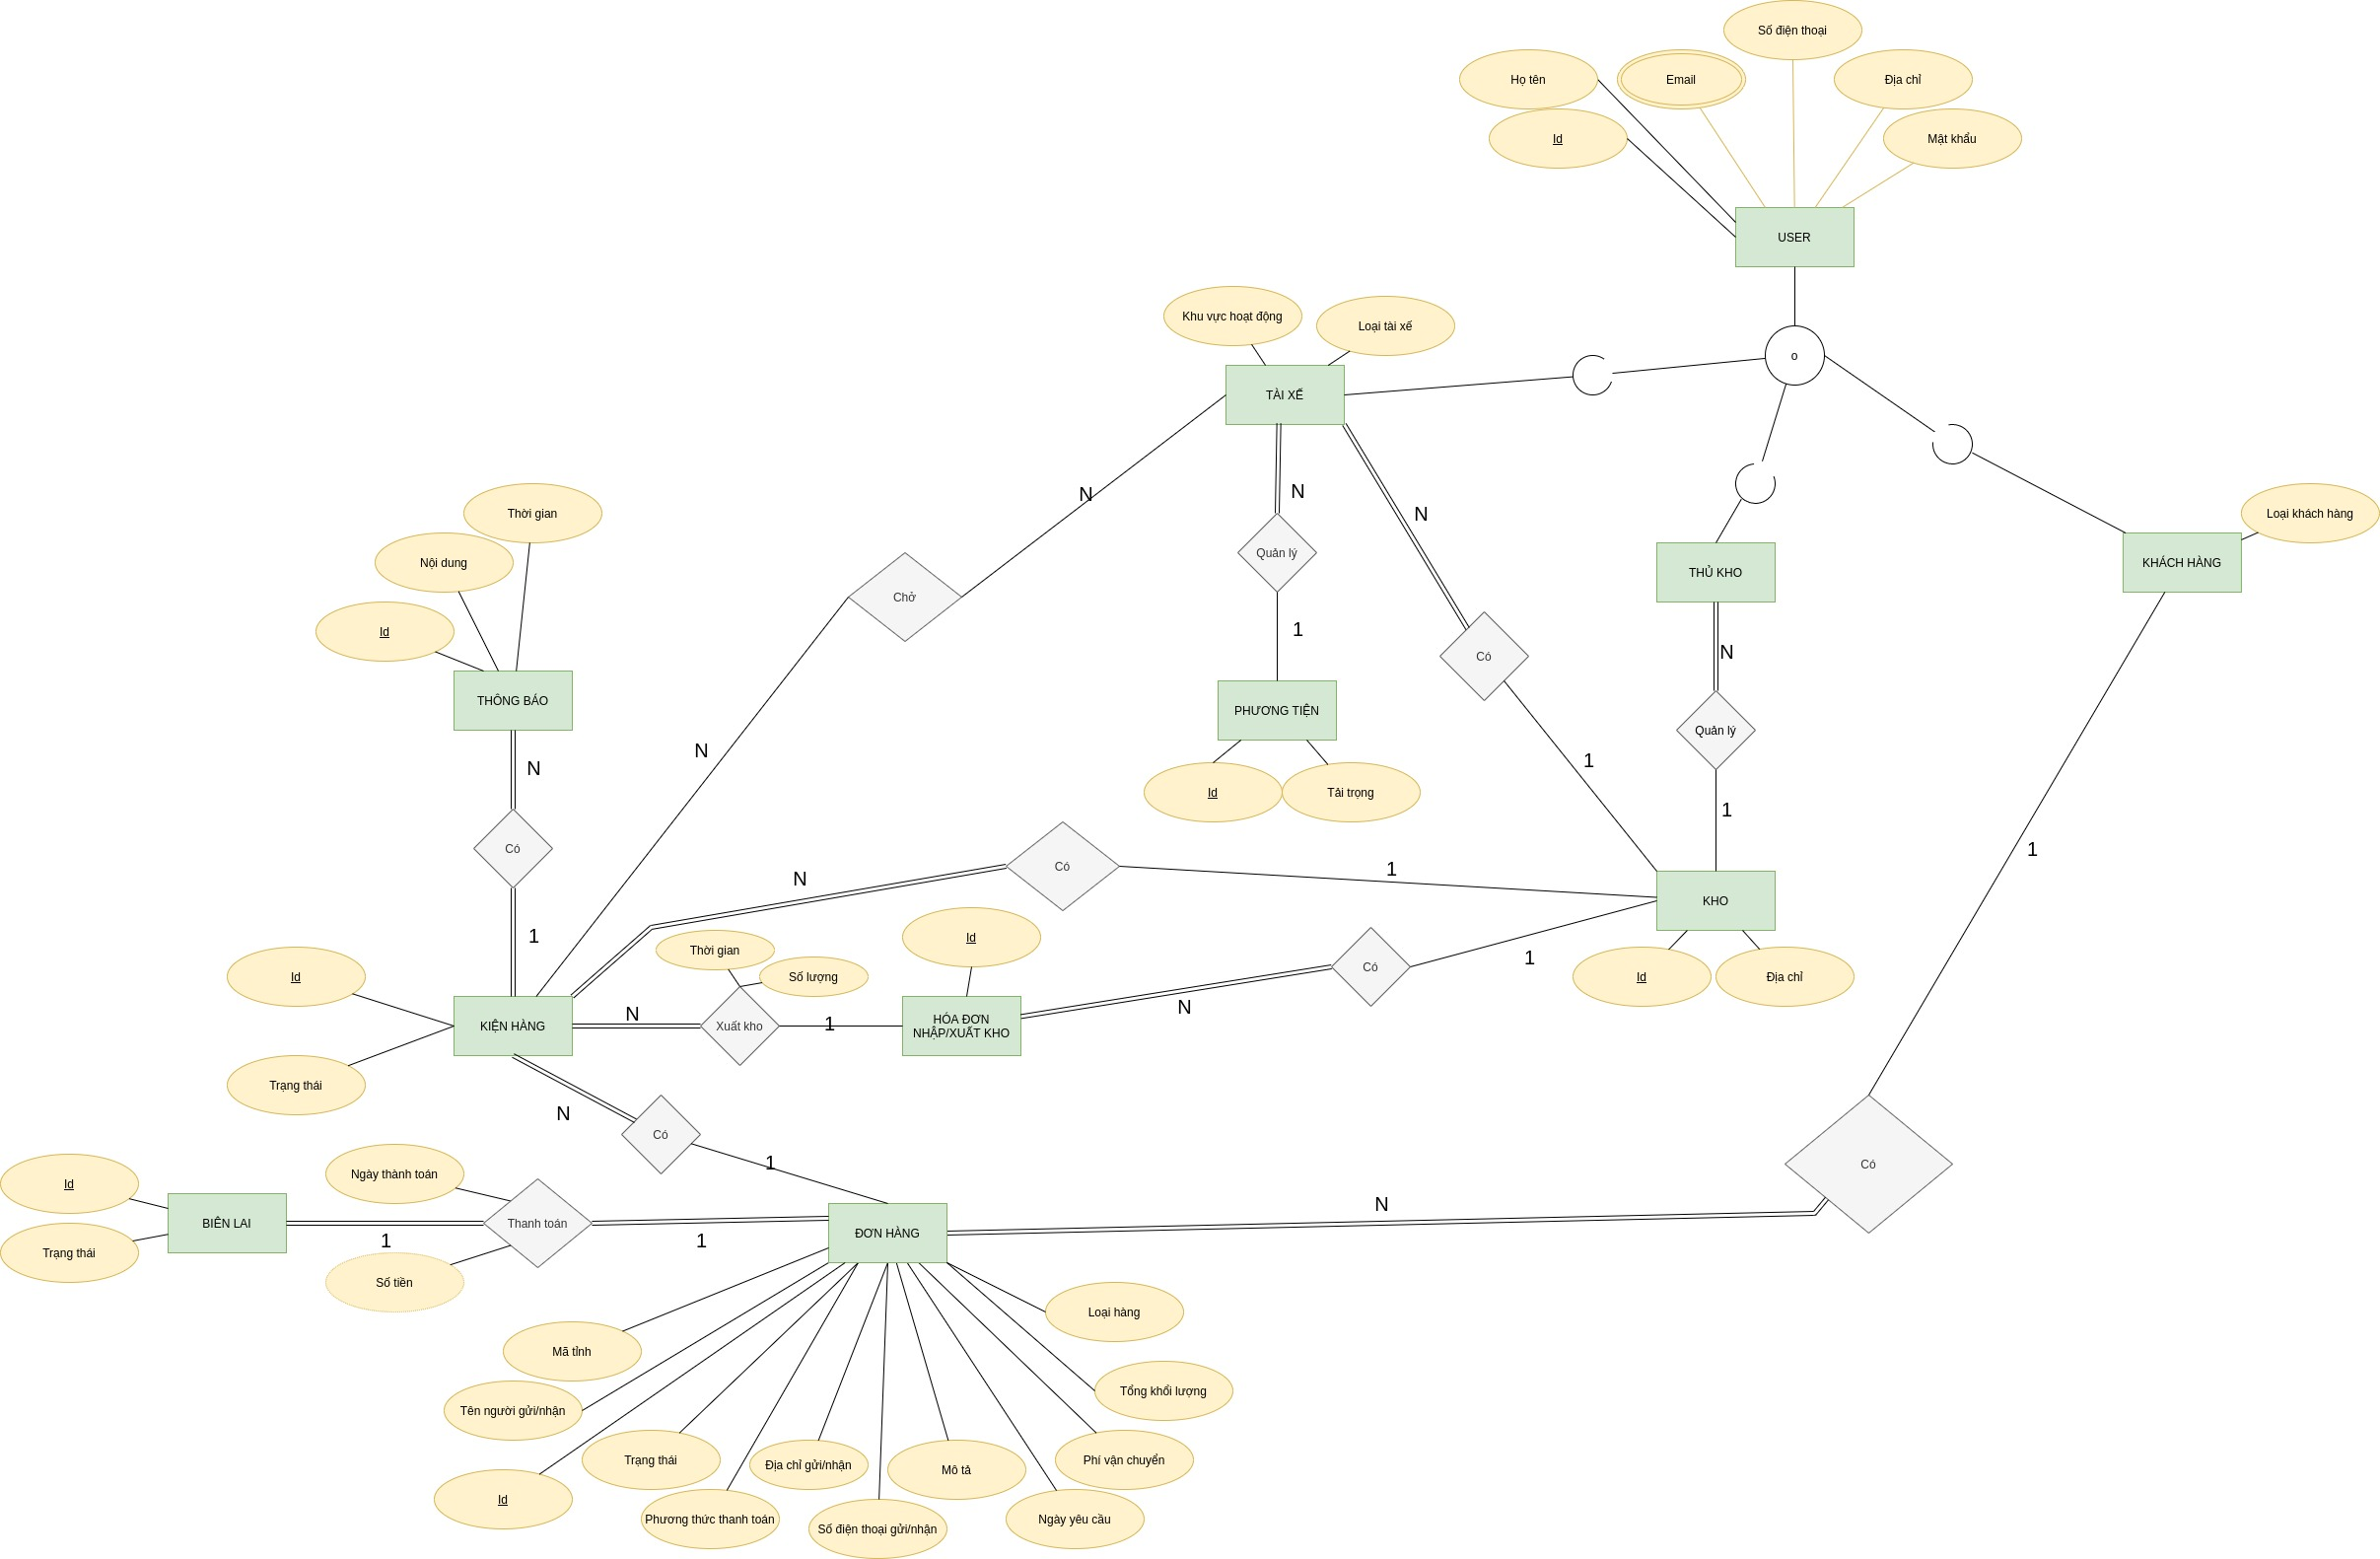
\includegraphics[angle=90, width=15cm, height=20cm]{Images/ERD.jpg}
			\centering
			\linebreak
			\caption{Lược đồ ERD}
		\end{figure}
	
	\newpage
	
	\newpage
	
	Sau khi thiết kế ERD nhóm tiến hành chuyển đổi thành các bảng tương ứng trong database như sau:
	
	\begin{itemize}
		\item \textbf{Order}
		
		\begin{table}[H]
			\centering\begin{tabular}{|l|m{30em}|}
				\hline 
				orderId & Mã đơn hàng\\
				\hline 
				assignedDrivers & Lưu danh sách tài xế đang được gán để đi lấy hàng \\ 
				\hline
				countcompletesuborder & Đếm số lượng kiện hàng đã hoàn tất \\
				\hline 
				driverIds & Danh sách các tài xế vận chuyển đơn hàng \\
				\hline
				fee & Phí vận chuyển \\
				\hline
				isDirectlyReceive & Người nhận có nhận trực tiếp hay không \\
				\hline
				isDirectlySend & Người gửi có gửi trực tiếp hay không \\
				\hline
				destStockId & Mã kho đích \\
				\hline
				detailOrder & Chi tiết đơn hàng \\
				\hline
				description & Mô tả đơn hàng \\
				\hline
				orderStatus & Trạng thái đơn hàng \\
				\hline
				orderTime & Thời gian tạo đơn hàng \\
				\hline
				paymentSide & Người thanh toán \\
				\hline
				paymentStatus & Trạng thái thanh toán \\
				\hline
				provinceCode & Mã tỉnh thành \\
				\hline
				remainWeight & Khối lượng còn lại \\
				\hline
				srcStockId & Mã kho nguồn \\
				\hline
				subOrderIds & Danh sách các kiện hàng tạo thành \\
				\hline
				totalWeight & Tổng khối lượng đơn hàng \\
				\hline
				userId & Mã khách hàng \\
				\hline
				value & Giá trị đơn hàng \\
				\hline
			\end{tabular}
			\caption{Schema Order}
		\end{table}
	
	\newpage
	
		\item \textbf{SubOrder}
		
		\begin{table}[H]
			\centering\begin{tabular}{|l|m{30em}|}
				\hline 
				subOrderId & Mã kiện hàng\\
				\hline 
				destDriverId & Mã tài xế đi giao \\ 
				\hline
				destDriverName & Tên tài xế đi giao \\
				\hline 
				destDriverPhone & Số điện thoại tài xế đi giao \\
				\hline
				destStockId & Mã kho đích \\
				\hline
				driverId & Mã tài xế đi lấy \\
				\hline
				driverName & Tên tài xế đi lấy \\
				\hline
				driverPhone & Số điện thoại tài xế đi lấy \\
				\hline
				externalDriverId & Mã tài xế liên tỉnh \\
				\hline
				externalDriverName & Tên tài xế liên tỉnh \\
				\hline
				externalDriverPhone & Số điện thoại tài xế liên tỉnh \\
				\hline
				issue & Nội dung vấn đề phát sinh \\
				\hline
				orderId & Mã đơn hàng \\
				\hline
				subOrderStatus & Trạng thái kiện hàng \\
				\hline
				provinceCode & Mã tỉnh thành \\
				\hline
				srcStockId & Mã kho nguồn \\
				\hline
				subOrderTime & Thời gian tạo kiện hàng \\
				\hline
				timeHistory & Danh sách thời gian update trạng thái đơn hàng \\
				\hline
				userId & Mã người dùng \\
				\hline
				weight & Khối lượng kiện hàng \\
				\hline
			\end{tabular}
			\caption{Schema SubOrder}
		\end{table}
	
	
	
		\item \textbf{ImportInfo}
		
		\begin{table}[H]
			\centering\begin{tabular}{|l|m{30em}|}
				\hline 
				id & Mã nhập kho\\
				\hline 
				driverId & Mã tài xế nhập kho\\ 
				\hline
				driverName & Tên tài xế nhập kho \\
				\hline 
				driverPhone & Số điện thoại tài xế nhập kho \\
				\hline
				importTime & Thời gian nhập kho \\
				\hline
				stockId & Mã kho \\
				\hline
				stockkeeperId & Mã thủ kho \\
				\hline
				stockkeeperName & Tên thủ kho \\
				\hline
				stockkeeperPhone & Số điện thoại thủ kho \\
				\hline
				subOrderIds & Danh sách kiện hàng nhập kho \\
				\hline
			\end{tabular}
			\caption{Schema ImportInfo}
		\end{table}
	
	\newpage
	
	
		\item \textbf{ExportInfo}
		
		\begin{table}[H]
			\centering\begin{tabular}{|l|m{30em}|}
				\hline 
				id & Mã xuất kho\\
				\hline 
				driverId & Mã tài xế xuất kho\\ 
				\hline
				driverName & Tên tài xế xuất kho \\
				\hline 
				driverPhone & Số điện thoại tài xế xuất kho \\
				\hline
				importTime & Thời gian xuất kho \\
				\hline
				stockId & Mã kho \\
				\hline
				stockkeeperId & Mã thủ kho \\
				\hline
				stockkeeperName & Tên thủ kho \\
				\hline
				stockkeeperPhone & Số điện thoại thủ kho \\
				\hline
				subOrderIds & Danh sách kiện hàng xuất kho \\
				\hline
			\end{tabular}
			\caption{Schema ExportInfo}
		\end{table}

	
		\item \textbf{SupportRequest}
		
		\begin{table}[H]
			\centering\begin{tabular}{|l|m{30em}|}
				\hline 
				id & Mã yêu cầu\\
				\hline 
				userId & Mã khách hàng\\
				\hline 
				orderId & Mã đơn hàng\\ 
				\hline
				reqTime & Thời gian yêu cầu \\
				\hline 
				content & Nội dung yêu cầu \\
				\hline
				emailAddress & Địa chỉ mail của khách hàng \\
				\hline
				reply & Thông tin phản hồi \\
				\hline
			\end{tabular}
			\caption{Schema SupportRequest}
		\end{table}
	
		\item \textbf{StatisticFee}
		
		\begin{table}[H]
			\centering\begin{tabular}{|l|m{30em}|}
				\hline 
				date & Ngày tháng năm theo format yyMMđd\\
				\hline 
				totalFee & Mã khách hàng\\
				\hline 
			\end{tabular}
			\caption{Schema StatisticFee}
		\end{table}
	
	
		\item \textbf{StatisticTrans}
		
		\begin{table}[H]
			\centering\begin{tabular}{|l|m{30em}|}
				\hline 
				date & Ngày tháng năm theo format yyMMđd\\
				\hline 
				transSuccess & Số đơn hàng thành công\\
				\hline 
				transCancel & Số đơn hàng bị hủy\\
				\hline 
				transFail & Số đơn hàng thất bại\\
				\hline 
			\end{tabular}
			\caption{Schema StatisticFee}
		\end{table}
	
	\newpage
	
		\item \textbf{Driver}
		
		\begin{table}[H]
			\centering\begin{tabular}{|l|m{30em}|}
				\hline 
				id & Mã tài xế\\
				\hline 
				area & Mã khu vực hoạt động của tài xế\\
				\hline 
				status & Trạng thái hoạt động của tài xế\\
				\hline 
				vehicleId & Mã phương tiện\\
				\hline 
			\end{tabular}
			\caption{Schema Driver}
		\end{table}
	
		\item \textbf{Role}
		
		\begin{table}[H]
			\centering\begin{tabular}{|l|m{30em}|}
				\hline 
				userId & Mã user\\
				\hline 
				role & Vai trò của user\\
				\hline 
			\end{tabular}
			\caption{Schema Role}
		\end{table}
	
		\item \textbf{Stocker}
		
		\begin{table}[H]
			\centering\begin{tabular}{|l|m{30em}|}
				\hline 
				id & Mã thủ kho\\
				\hline 
				areaId & Mã kho\\
				\hline 
			\end{tabular}
			\caption{Schema Stocker}
		\end{table}
	
		\item \textbf{User}
		
		\begin{table}[H]
			\centering\begin{tabular}{|l|m{30em}|}
				\hline 
				id & Mã user\\
				\hline 
				address & Địa chỉ\\
				\hline 
				email & Email\\
				\hline 
				password & Mật khẩu\\
				\hline 
				phone & Số điện thoại\\
				\hline 
				provinceCode & Mã tỉnh\\
				\hline 
				username & Tên tài khoản\\
				\hline 
			\end{tabular}
			\caption{Schema User}
		\end{table}
	
		\item \textbf{Vehicle}
		
		\begin{table}[H]
			\centering\begin{tabular}{|l|m{30em}|}
				\hline 
				id & Mã phương tiện\\
				\hline 
				currentWeight & Trọng tải hiện tại\\
				\hline 
				totalWeight & Trọng tải\\
				\hline 
				number & Biển số\\
				\hline 
			\end{tabular}
			\caption{Schema Vehicle}
		\end{table}
	
	\newpage
	
		\item \textbf{Warehouse}
		
		\begin{table}[H]
			\centering\begin{tabular}{|l|m{30em}|}
				\hline 
				id & Mã kho\\
				\hline 
				address & Địa chỉ kho\\
				\hline 
				areaCode & Mã khu vực\\
				\hline 
			\end{tabular}
			\caption{Schema Warehouse}
		\end{table}


	\end{itemize}



	



	